\section {Event selection}
\label{sec:GBJ1:EvtSel}
\subsection{Data Samples}
The analysis was performed on 7 TeV pp collision data that was recorded between April and October 2010 using the ATLAS detector with a centre-of-mass energy of 7 TeV. 
Data was only used if it was collected during stable beam conditions and there was good data quality. 
The data quality was assessed by checking that all the parts of the detector and trigger were performing normally, and the physics objects (eg jets and muons) were being correctly reconstructed. *need to explain how this was checked*

\subsection{Trigger Strategy}
The trigger strategy used the ATLAS jet triggers to select events, for the analysis, required that certain triggers fired for specific dijet topologies. 
During the data periods B-D only the level 1 jet triggers were also used for selecting events, and during periods E-I the level 2 jet triggers were used. 
There are three different trigger areas in the ATLAS detectors, two in the large rapidity region (one forward, $\eta>3.2$ and one backwards, $\eta<-3.2$) and one in the central region ($|\eta|<3.2$). 
In the trigger strategy only the central trigger region is used. 

The L1 jet triggers have names of the format $\rm L1\_JX$, where X is the EM transverse energy threshold.
The format of the L2 jets are .*Check exactly how the L2 name relates to L1*
 
The trigger that is required to be satisfied depends on what $\bar{p_T}$ region the event falls into, and which data period it was collected in. 
Table \ref{tab:trig_strat} shows the trigger requirement for different $\bar{p_T}$ regions and data periods.

\begin{table}[htdp]
\centering
\begin{tabular}{ | c | c | c | c | }
  \hline                       
 $\bar{p_T}$ [GeV] & Period B-D & Period E-F & Period G-I \\
  \hline                       
50 - 70   & $\rm L1\_J5$  & $\rm EF\_j20\_jetNoCut$ & $\rm EF\_j20\_jetNoEF$ \\
70 - 90   & $\rm L1\_J10$ & $\rm EF\_j30\_jetNoCut$ & $\rm EF\_j30\_jetNoEF$ \\
90 - 120  & $\rm L1\_J15$ & $\rm EF\_j35\_jetNoCut$ & $\rm EF\_j35\_jetNoEF$ \\
120 - 150  & $\rm L1\_J30$ & $\rm EF\_j50\_jetNoCut$ & $\rm EF\_j50\_jetNoEF$ \\
150 - 180  & $\rm L1\_J55$ & $\rm EF\_j75\_jetNoCut$ & $\rm EF\_j75\_jetNoEF$ \\
180 - 210  & $\rm L1\_J75$ & $\rm EF\_j95\_jetNoCut$ & $\rm EF\_j95\_jetNoEF$ \\ 
210 - 7000  & $\rm L1\_J95$ & $\rm EF\_L1J95\_NoAlg$  & $\rm EF\_L1J95\_NoAlg$ \\
  \hline                       
\end{tabular}
\caption{L1 and L2 jet triggers used to select events. Jet triggers are shown for different $\bar{p_T}$ regions and data periods. \label{tab:trig_strat}}
\end{table}%

\subsection{Noise and Pileup Rejection}
Events are rejected if there is any jet with $p_T>20$ GeV which is found as either ``bad" (jet not resulting from a real energy deposit) or ``ugly" (real energy deposit but measured poorly) as defined by the jet cleaning definitions. 

%UGLY JETS
Ugly jets are those that are badly measured but are associated with real energy deposits.
Ugly jets are often found in regions between detectors ``cracks", where the performance of the detectors are not optimal (see section on detects). 
The two cuts that are applied to remove ugly jets are, 
$frac_{TileGap3}>0.5$ where $frac_{TileGap3}$ is the *need to check definition*, and $frac_{BadCell}>0.5$ where $frac_{BadCell}$ is the fraction of the electro-magnetic energy of the jet that comes from bad cells inside the jet.

%BAD JETS
Bad jets are jets that are not associated with a real energy deposit. 
Bad jets can come from a variety of different sources, the more significant are cosmic and beam background, HEC spikes and EM coherent noise. 
The two different definitions of bad jets used to cut are, loose and medium, where medium includes the loose cuts, but also applies stricter ones.
The variables used for the two different bad jets definitions are:

\begin{itemize}
  \item The jet charge fraction, \Bold{Chf}, is the ratio of the sum of the \pt{} of tracks associated to the jet to the calibrated jet \pt{}.  
  \item \Bold{EMf} is the fraction of the jet EM scale energy that comes from EM clusters *Check this and definition of EM clusters*
  \item \Bold{HECf} is the fraction of the jet energy that was measured in the HEC. 
  \item The LAr quality, \Bold{LArQ}, is the fraction of the jet energy coming from LAr cells with a cell Q-factor$>$4000. *Need to define Q-factor* 
  \item The HEC quality, \Bold{HECQ}, is the fraction of the jet energy coming from HEC cells with a cell Q-factor$>$XXX (what is the hec value). *Need to define Q-factor* 
  \item \Bold{neg. E} is the sum of the negative energy cells in the jet.
  \item Jet time, \Bold{t}, is computed as the energy squared cells mean time *Check this and make it better*
  \item \Bold{FMax} is the maximum energy fraction in one calorimeter layer.
\end{itemize}


The definition for the loose and medium jet cleaning cuts is shown in Figure \ref{GBJ1:JetCleanRel16}. 
Cutting on the medium definition removes a higher proportion of bad jets than the loose definition, but the efficiency for real jets is also lower.
The effects of the jet cleaning cuts and the justification for using the loose bad jet requirement is shown in Section \ref{sec:GBJ1:Pileup}.


\begin{figure}
  \centering
  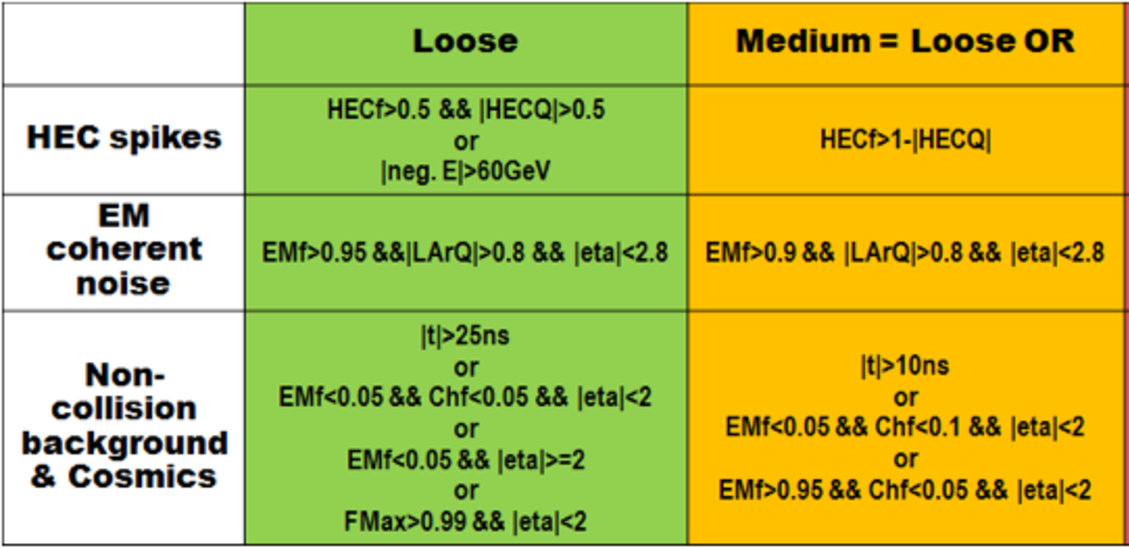
\includegraphics[width=0.9\textwidth]{figures/GBJ1/JetCleaning/JetCleaningRel16.pdf}
  \caption{Definition of the loose and medium bad jet definitions.}
\label{GBJ1:JetCleanRel16}
\end{figure}


Events are only used if the number of reconstructed primary vertices is equal to one.
This cut reduces the impact of in-time pile-up. 
In-time pileup is defined as multiple proton-proton interactions in the same bunch crossing and results in addition primary vertices.
The cut is necessary to remove the impact of extra energy deposits in the rapidity region between the boundary jets, which can degrade the gap by either producing a new jet, or by increasing the \pt{} of an existing jet to greater than \qz{}.

Out-of-time pileup also adds extra energy into the detector, and thus effect the gap fraction. 
Out-of-time pileup is additional energy coming from previous bunch collisions and depends on both the number of primary vertices of the previous bunches and the bunch spacing. 

The residual effect of in-time pileup and out-of-time pileup is studied in Section \ref{sec:GBJ1:Cleaning}. 


%As described in section XXX, there are two types of pileup; in-time pileup and out-of-time pileup. Both forms of pileup add additional energy into the detectors, and can add additional energy into existing jets, or even add new jets. The additional energy from the pileup interactions can change the gap fraction and mean number of jets distributions.  In this section the effect of both in-time and out-of-time pileup will be determined, and the effectiveness of the pileup cut outlined in section \ref{sec:GBJ1:EvtSel} will be assessed.

%In-time pileup is due to multiple proton-proton interactions in the same bunch collision. In-time pileup can be estimated by looking at the number of reconstructed primary vertices. 




%-The data used
%-GRL explanation
%-Trigger
%-pileup cut
%-fake jets removed




